\documentclass{article}
\usepackage{graphicx}
\usepackage[T2A]{fontenc}
\usepackage{listings}
\usepackage{float}
\usepackage{geometry}
\usepackage[english, russian]{babel}
\usepackage{indentfirst}
\usepackage{setspace}
\usepackage{tikz}
\usepackage{amsmath}
\usepackage{amssymb}
\usepackage{tocbibind}
\usepackage[style=gost-numeric,sorting=none]{biblatex}
\addbibresource{bibliography.bib}

\setstretch{1.25} 
\geometry{
  a4paper,
  left=2cm,
  right=2cm,
  top=2cm,
  bottom=2cm
}

\title{Pres}
\author{Gregory Of Lebennin}
\date{October 2024}

\begin{document}

\tableofcontents

\section{Постановка задачи}

\subsection{Описание физической задачи}
Основная задача: моделирование процессов образования и свойств частиц для эксперимента NICA. Для такого моделирования необходимо создать модель, описывающую основные свойства как лёгких, так и тяжелых мезонов. Для этого будет использоваться модель с нелокальными взаимодействиями.

Суть модели состоит в том, что образование мезонов (как кварк-антикварковых пар) сопровождается обменом глюонов, однако обмен глюонов не описывается с помощью суммирования диаграм, так как теория возмущений неприменима (разложение по малой константе связи невозможно).

\begin{figure}[H]
    \centering
    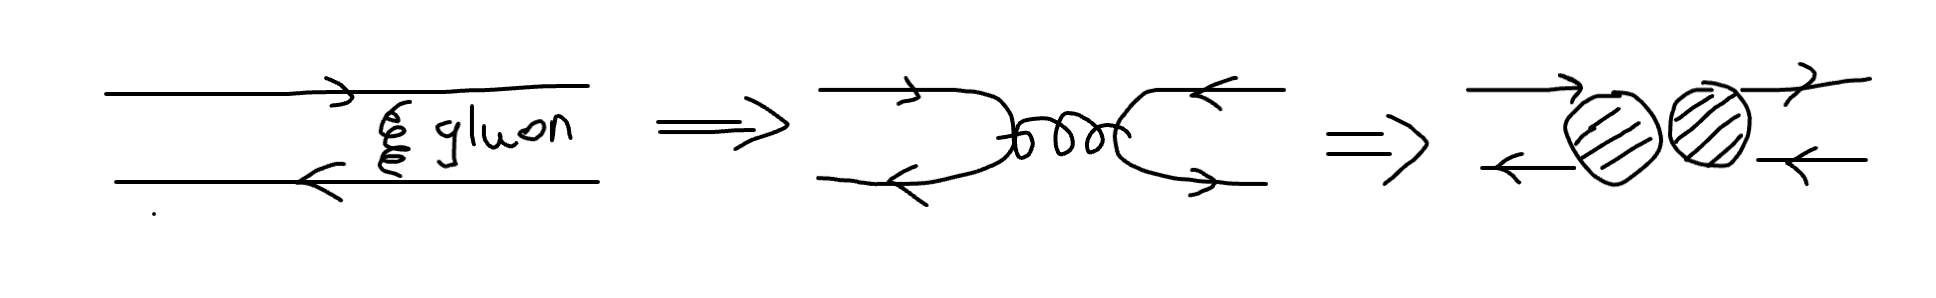
\includegraphics[width=0.5\textwidth]{interaction.png}
\end{figure}

Назовём \tikz \fill[black] (0,0) circle [radius=1.ex]; форм-фактором и будем использовать модель Гаусовского типа 
\begin{equation}
    F(p^2)=exp[\frac{-p^2}{\lambda^2}]
\end{equation}
так что размер форм-фактора будет определяться описанной $F(p^2)$. Для описания частиц нам требуется знать массы, константы распадов и процесс распадов.

\begin{figure}[H]
    \centering
    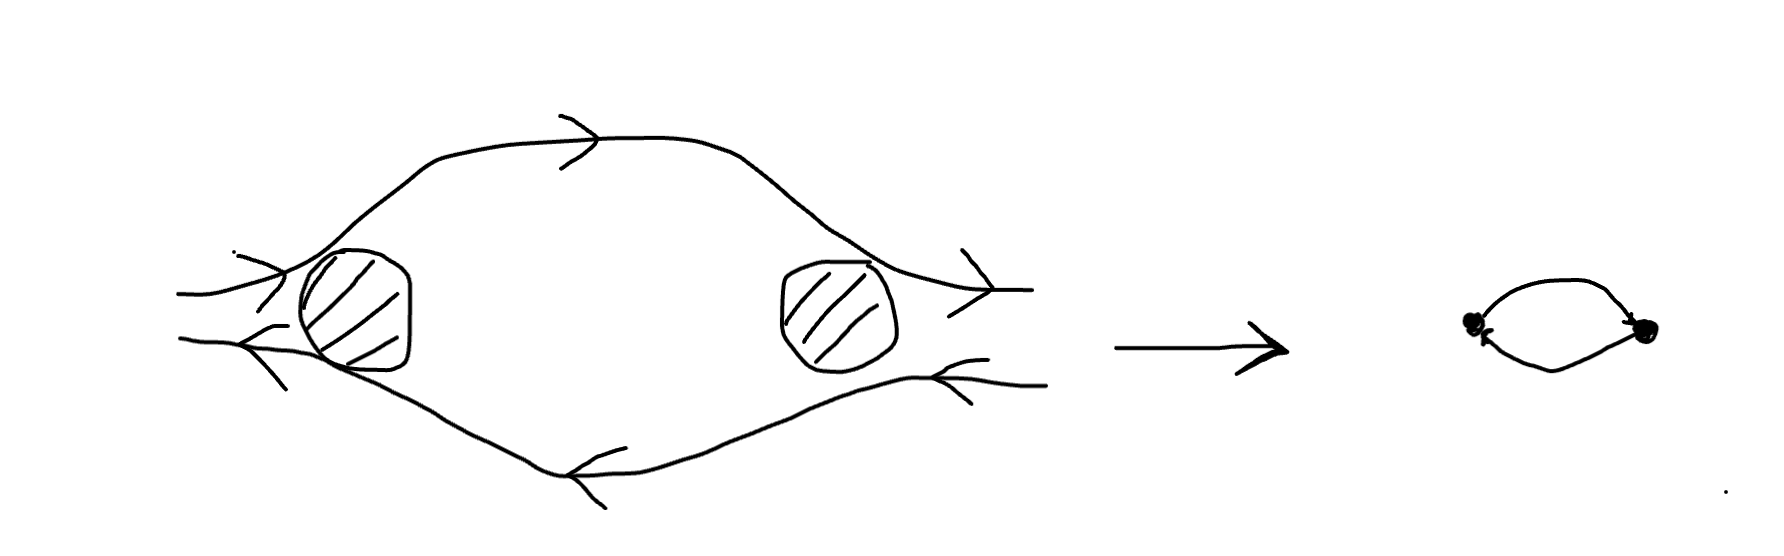
\includegraphics[width=0.5\textwidth]{mases.png}
\end{figure}

\begin{equation}
    \tikz[baseline=-0.5ex]{
    \filldraw (0, 0) circle (0.1cm);
    \filldraw (1, 0) circle (0.1cm);
    \draw[->, thick] (0.1, 0.05) to[out=45, in=135] (0.9, 0.05);
    \draw[<-, thick] (0.1, -0.05) to[out=-45, in=-135] (0.9, -0.05);
} + \tikz[baseline=-0.5ex]{
    \filldraw (0, 0) circle (0.1cm);
    \filldraw (1, 0) circle (0.1cm);
    \draw[->, thick] (0.1, 0.05) to[out=45, in=135] (0.9, 0.05);
    \draw[<-, thick] (0.1, -0.05) to[out=-45, in=-135] (0.9, -0.05);
}\tikz[baseline=-0.5ex]{
    \filldraw (0, 0) circle (0.1cm);
    \filldraw (1, 0) circle (0.1cm);
    \draw[->, thick] (0.1, 0.05) to[out=45, in=135] (0.9, 0.05);
    \draw[<-, thick] (0.1, -0.05) to[out=-45, in=-135] (0.9, -0.05);
} + ... = \frac{1}{1 - \tikz[baseline=-0.5ex]{
    \filldraw (0, 0) circle (0.1cm);
    \filldraw (1, 0) circle (0.1cm);
    \draw[->, thick] (0.1, 0.05) to[out=45, in=135] (0.9, 0.05);
    \draw[<-, thick] (0.1, -0.05) to[out=-45, in=-135] (0.9, -0.05);
}} 
\end{equation}

\begin{equation}
    \tikz[baseline=-0.5ex]{
    \filldraw (0, 0) circle (0.1cm);
    \filldraw (1, 0) circle (0.1cm);
    \draw[->, thick] (0.1, 0.05) to[out=45, in=135] (0.9, 0.05);
    \draw[<-, thick] (0.1, -0.05) to[out=-45, in=-135] (0.9, -0.05);
} \to \int_{0}^{\infty}\frac{dp}{2\pi^4}\{F(p^2)\frac{1}{u_1u_2}\} = \int_{0}^{\infty}\frac{dp}{2\pi^4}\{\frac{1}{[(p + q_1)^2 + m_1^2][(p + q_2)^2 + m_2^2]}\}.
\end{equation}

Для расчета данных интегралов используются формулы:

\begin{equation}
    \frac{1}{(p + q_1)^2 + m_1^2} = \int_{0}^{\infty}dt\{exp(-t[(p + q_i)^2 + m_i^2])\}
\end{equation}
\begin{equation}
    F(p^2) = \int_{0}^{\infty}ds\{exp(-sp^2)F(s)\}
\end{equation}

Случаи взаимодействия более чем двух мезонов

\begin{figure}[H]
    \centering
    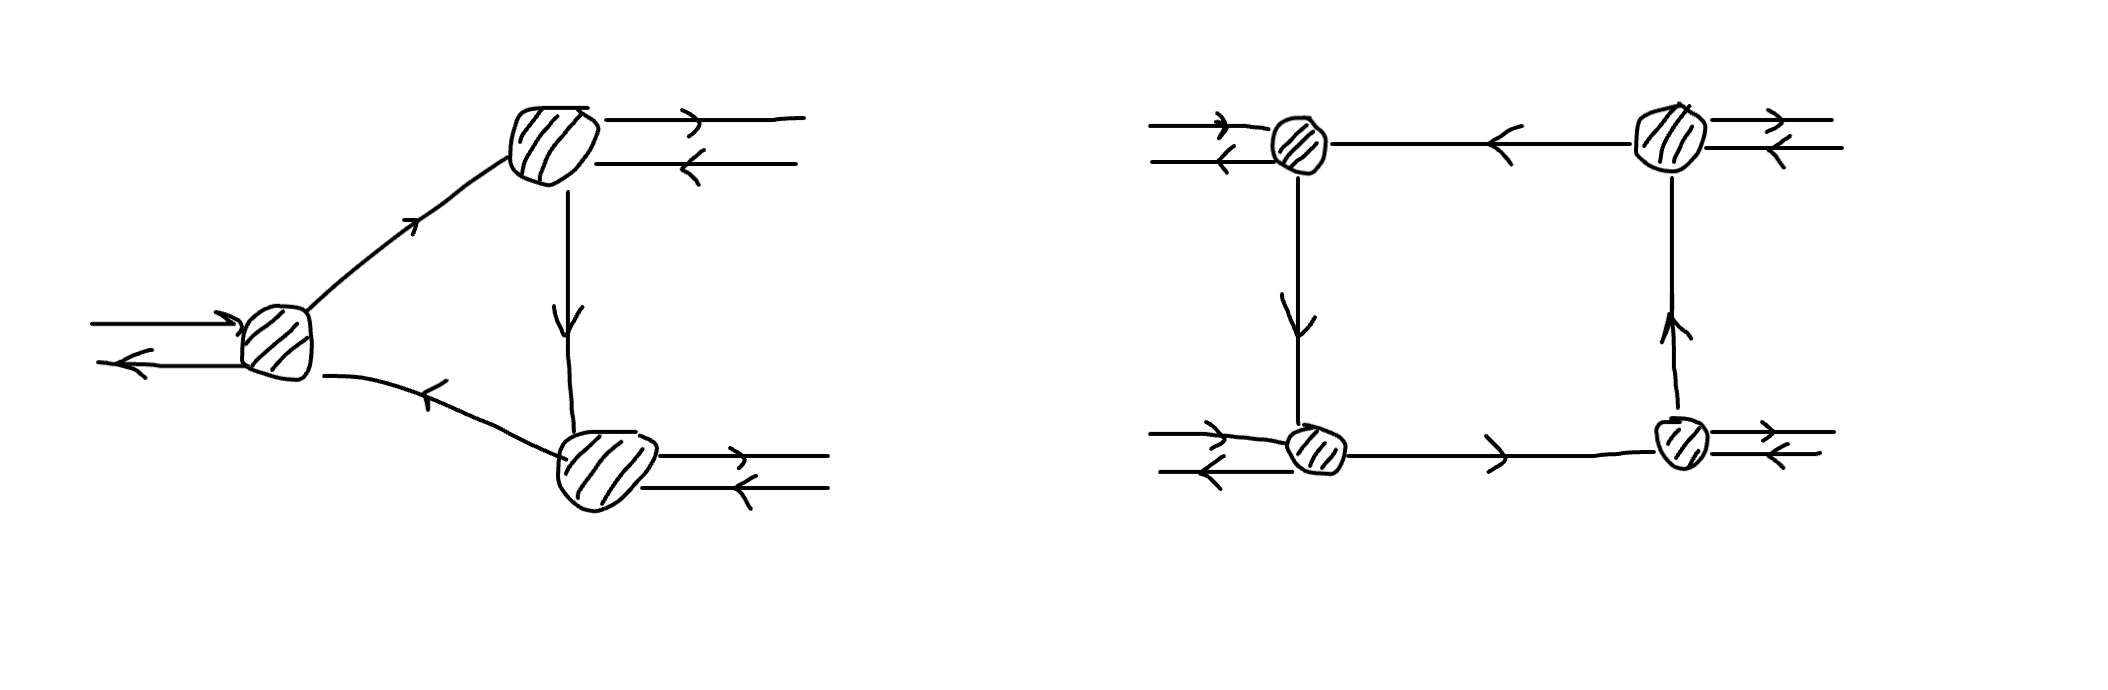
\includegraphics[width=0.5\textwidth]{multiple-interactions.png}
\end{figure}

описываются трех- и четырёхкратными интегралами. 

Амплитуды конкретных распадов и их квадраты будут вычисляться с помощью программы аналитических вычислений FORM. Основной проблемой данной задачи является исчисление многократных интегралов.

\subsection{Постановка математической задачи}

Классические численные методы интегрирования зачастую оказываются неэффективными при интегрировании функций многих переменных в связи с чем ставится задача разработать нейросеть-аппроксиматор $\hat{f}(X), |X| \geq 4$ подынтегральной функции $f(X)$ интеграла $I(f)$ вида: 
\begin{equation}
    I(f) = \int_{S}^{}dX\{f(X)\}
\end{equation}
такую, что она будет обеспечивать погрешность не более $\varepsilon$:
\begin{equation}
   |f(X) - \hat{f}(X)| < \varepsilon 
\end{equation}
и численный интеграл вида:
\begin{equation}
    \hat{I}(f) = \int_{S}^{}dX\{\hat{f}(X)\}
\end{equation}
будет иметь погрешность не более некоторой $\epsilon$:
\begin{equation}
    |I(f) - \hat{I}(f)| < \epsilon.
\end{equation}

В частности, в случае, если $\hat{f}(X)$ имеет архитектуру многослойного перцептрона (MLP), её можно выразить в виде нелинейной функции:
\begin{equation}
    \hat{f}(X) = b^{(2)} + W^{(2)T}\phi(b^{(1)}+W^{(1)}X),
\end{equation}

где $\phi($•$)$ - функция активации нейронов \textit{логистическая сигмоида},

$b^{(1)}, b^{(2)}, W^{(1)}, W^{(2)}$ - смещения и веса нейронной сети.

Таким образом, сложная подынтегральная функция $f(X)$ не имеющая аналитического решения аппроксимируется нейронной сетью $\hat{f}(X)$, интеграл которой равен:

\begin{equation}
    \hat{I}(f) = b^{(2)}\prod_{i=1}^{n}(\beta_i - \alpha_i) + \sum_{j=1}^{k}w_j^{(2)}[\prod_{i=1}^{n}(\beta_i - \alpha_i) + \frac{\Phi_j}{\prod_{i=1}^{n}w_{ij}^{(1)}}]
\end{equation}

\begin{equation}
    \Phi_j = \sum_{r=1}^{2^n}\xi_{r}Li_n(-exp[-b_j^{(1)} - \sum_{i=1}^{n}w_{ij}^{(1)}l_{i,r}])
\end{equation}

\begin{equation}
    \xi_{r} = \prod_{d=1}^{n}(-1)^{[{r}/{2^{n-d}}]}
\end{equation}

\begin{equation}
    l_{i,r} = \left\{
\begin{array}{ll}
\alpha_i, & \text{если } [{r}/{2^{n-d}}] \% 2 = 0 \\
\beta_i, & \text{если } [{r}/{2^{n-d}}] \% 2 \neq 0
\end{array}
\right.
\end{equation}

\section{Задачи}

\begin{enumerate}
    \item анализ существующих архитектур нейросетей, которые подходили бы для аппроксимации подынтегральных функций многих переменных.
    \item подбор методов оптимизации нейросетей, таких как алгоритм Левенберга-Марквардта (LMA), алгоритм Adam и другие
    \item построение конфигурации из нейросети-аппроксиматора (НСА) на основе полученных ранее данных и функции – численного интегратора (ЧИ)
    \item проверка функционирования ЧИ на основе вычисленных иными методами интегралов из физической задачи, сформулированной профессором Калиновским Ю. Л.
    \item доработка НСА и ЧИ
    \item создание пакета нейросетевого численного интегрирования на основе НСА и ЧИ
    \item применение полученного пакета для численного интегрирования интегралов из физической задачи, сформулированной профессором Калиновским Ю. Л., и в других задачах
\end{enumerate}



\section{Теория}

\subsection{Численное интегрирование}

Задача численного интегрирования сводится к вычислению некоторого значения $I(f) \in \mathbb{R}$ от некоторой функции $f: \mathbb{R}^n \rightarrow \mathbb{R}$ над гиперплоскостью $S$:

\begin{equation}
    \hat{I}(f) = \int_{S} f(X) \, dX,
\end{equation}

причём $|X| = n$.

Для случаев, когда число аргументов функции $f(X): n = 1$ разработано большое количество численных методов интегрирования, которые обеспечивают значительную точность. Однако при увеличении числа измерений многие методы становятся неэффективными, неточными или неприменимыми в силу феномена, получившего название "проклятие размерности". Одним из способов решения данной проблемы является использование методов разреженных сеток, другим - использование методов группы Монте-Карло. Однако первый способ показывает низкую эффективность, а второй - в силу своей стохастической природы - вынуждает оперировать вероятностной оценкой значений численного интеграла, из чего следует, что как значения, так и ошибки могут варьироваться от вычисления к вычислению. \cite{lloyd2020using  }

\subsection{Анализ предметной области 1}

Анализ предметной области был начат со статьи Ллойда, Стеффана и Ирани, которая посвящена нейросетевому подходу в численном интегрировании. На основе этой статьи были выделены архитектура \textit{MLP} (\textit{Multi-Layer Perceptron}) и алгоритм оптимизации \textit{Adam}. \cite{lloyd2020using}

В вышеупомянутой статье авторы предлагают использовать алгоритм оптимизации Левенберга-Марквардта, который на самом деле показывает себя быстро сходящимся и эффективным для задачи оптимизации нелинейной системы, которой и является нейросеть-аппроксиматор. Однако, на первой итерации разработки было отдано предпочтение алгоритму Adam, так как он один из самых эффективных алгоритмов оптимизации нейронных сетей из присутствующих в библиотеках PyTorch и Tensorflow. \cite{lloyd2020using}\cite{roweis1996levenberg}\cite{yan2021adaptive}\cite{huang2023optimization}

\large{ПОДУМАЙ ПРО ТО, КАК ИМЕННО ЭТО ВСЁ ЗВУЧИТ И НУЖНО ЛИ ТАКОЕ ОПИСАНИЕ}

В дальнейшем планировалось произвести более глубокий анализ для выявления возможных архитектур и алгоритмов оптимизации.

\subsection{Первый интеграл}

\begin{equation}
    \int_{0}^{1}d\alpha\{\alpha^{a}(1 - \alpha)^b\}\int_{0}^{\infty}dt\{\frac{t^m}{(1+t)^n}F[z_{0}]\} \equiv I(a, b, m, n; F[z_{0}])
\end{equation}
\begin{equation}  
    F[z_0] = exp[-2z_0]
\end{equation}
\begin{equation} 
    z_0 = tD + \frac{t}{1 + t}R^2
\end{equation}
\begin{equation}     
    D = \alpha_1(b_1^{2}P^2 + m_1^2) + \alpha_2(b_2^{2}P^2 + m_2^2)
\end{equation}
\begin{equation} 
    R^2 = (\alpha_1^{2}b_1^2 + \alpha_2^{2}b_2^2 + 2\alpha_{1}\alpha_{2}(m_{1}m_2))
\end{equation}
\begin{equation} 
    b_1 = -\frac{m_1}{m_1 + m_2}
\end{equation}
\begin{equation} 
    b_2 = \frac{m_1}{m_1 + m_2}
\end{equation}

\printbibliography[
heading=bibintoc,
title={Список использованной литературы}
]

\end{document}
